\documentclass[11pt]{article}

\setlength\parindent{0pt}
\setlength{\parskip}{.25\baselineskip}

\usepackage{fullpage}
\usepackage{hyperref}
\hypersetup{colorlinks=true}
\usepackage{amsmath,amsfonts,amssymb,bbm}
\usepackage{todonotes}
\usepackage{subcaption}
\usepackage[round]{natbib}   % omit 'round' option if you prefer square brackets
\usepackage[normalem]{ulem}

\DeclareMathOperator{\Tr}{Tr}
\newcommand{\R}{\mathbbm{R}}
\newcommand{\mba}{\mathbf{a}}
\newcommand{\mbb}{\mathbf{b}}
\newcommand{\mbx}{\mathbf{x}}
\newcommand{\mbxt}{\tilde{\mathbf{x}}}
\newcommand{\Sigmat}{\tilde{\Sigma}}
\newcommand{\mbz}{\mathbf{z}}
\newcommand{\mbw}{\mathbf{w}}
\newcommand{\mcN}{\mathcal{N}}
\newcommand{\mcP}{\mathcal{P}}
\newcommand{\eps}{\epsilon}
\newcommand{\trans}{\intercal}
\newcommand{\Ut}{\tilde{U}}
\DeclareMathOperator*{\argmax}{arg\,max}
\newcommand{\angstrom}{\text{\normalfont\AA}}
\newcommand{\red}[1]{\textcolor{red}{#1}}
%\newcommand{\todo}[1]{\textcolor{red}{TODO: #1}}


\title{Quasar Photo-z Research Notes}
%:  Stochastic Process Model for Semi-supervised \\Inference of Red Shift from Quasar Photometry} 
\author{Andrew Miller, Albert Wu, Ryan Adams, David Schlegel}
\date{\today}

%% DOC START
\begin{document}
\maketitle
\begin{abstract}
%We present a method to measure the red-shift of quasars from photometric observations.  Our method treats the unknown spectrum of a quasar as a latent stochastic process and uses statistical inference to infer the unknown structure.  Our model leverages a small number of existing examples of full quasar spectra with known red-shift to build a structured stochastic process prior distribution over unknown spectra.  We then use Bayesian inference to infer red-shift from a typical 5-band photometric sample of astronomical imagery, the so called ``photo-z'' problem.  
\end{abstract}

%\tableofcontents

\section{TODO}

\subsection{Data wrangling} 
\begin{itemize} \itemsep 0pt
\item \sout{ Download the DR10QSO dataset (\href{http://data.sdss3.org/datamodel/files/BOSS_QSO/DR10Q/DR10Q.html}{link}) to get PLATE-MJD-FIBER information. } (in DESIMCMC/data/DR10QSO)
\item \sout{ Download PLATE-MJD-FIBER files corresponding to quasars in DR10QSO dataset (note - these files contain red-shift, fluxes, pretty much everything \href{http://data.sdss3.org/datamodel/files/BOSS_SPECTRO_REDUX/RUN2D/spectra/PLATE4/spec.html}{spec-PLATE-MJD-FIBER files}).  Instructions in ``\href{https://www.sdss3.org/dr10/data_access/bulk.php}{optical spectra per file}'' section. } Script written, downloads need to happen on edison.  
\item 
\item See how the different plates sample different inputs.  Sinc resample to a common basis.  
\item Figure out how to normalize the spectra  
\end{itemize}

\subsection{Implementing}
\begin{itemize} \itemsep 0pt
\item \sout{write function spectrum to flux integration:}
  \begin{align}
    f_u, f_g, f_r, f_i, f_z 
      &= g(spec) \\
      &= g(\mathbf{w}) \text{ for spec weights/cluster } \mathbf{w}
  \end{align}
  where fluxes end up in nanomaggies.  Verify this with a few spec-PLATE-MJD-FIBER files (which has SPECTROFLUX and SPECTROSYNFLUX)
  
\item Implement rescaling, we have 
  \begin{align}
    f^{(rest)}(\cdot) 
      &= \ell \cdot f^{(sed)}(\cdot) & \text{ s.t. } \int f^{(sed)}(d\lambda) = 1 \\
      &= \ell \sum w_k B_k(\cdot)  & \text{ s.t. } \int B_k(\cdot) = 1, \sum w_k = 1 \\
    f^{(obs)}(\lambda) &= \ell^{(obs)} f^{(sed)}(\lambda \cdot( 1 + z)) & \text{ red-shift rescales, but sed is invariant }
  \end{align}
  That is, a \emph{luminosity-distance} value that scales the overall density, and a spectral energy density (SED) that integrates to 1.    

\item \sout{Implement smooth-ish LGCP prior over $B_k(\cdot)$ in pre-train optimization.}

\item \sout{Run the basis maximization code with these two formulations.}

\item Write a density estimator for the weights (or log weights) and use this in inference.  

\end{itemize}


\subsection{Experiments}
\begin{itemize} \itemsep 0pt
\item \sout{Basis smoothing - there is no smoothing along similar frequencies.  However there is clearly structure there.}
    \begin{itemize}
    \item \sout{Proper process model: try a Gaussian process with fixed covariance function - maybe an OU process or a matern initially.}
    \end{itemize}
\item Figure out an idea of the curvature at the MAP.  
\item Assess mixing of weights, z (and eventually basis) - I think it's mixing rather slowly...
\item Also, figure out what the Planck's law luminosity, temperature, radius degree of freedom issue. 

\item Inferences with structured prior over $w$'s and without.  Is there a difference in MSE or $\Delta z$?  A difference in Bayesian credible coverage? 
\end{itemize}

\subsection{Notes on SDSS data}
\begin{itemize} \itemsep 0pt
\item Spectra data access: \href{https://www.sdss3.org/dr10/spectro/spectro_access.php}{spectra data access information}
\item DR10QSO, \href{http://data.sdss3.org/datamodel/files/BOSS_QSO/DR10Q/DR10Q.html}{data model}.  Notes: 
  \begin{itemize}
  \item BOSS spectra files (latest, i believe) have spAll fields in in HDU 2 (\href{http://data.sdss3.org/datamodel/files/BOSS_SPECTRO_REDUX/RUN2D/spAll.html}{details here})
  \item The psfflux fields should carry over from the ``\href{http://data.sdss3.org/datamodel/files/BOSS_PHOTOOBJ/RERUN/RUN/CAMCOL/photoObj.html}{photoObj}'' field types
  \item the ``Z'' field should carry over from the ``\href{http://data.sdss3.org/datamodel/files/BOSS_SPECTRO_REDUX/RUN2D/PLATE4/RUN1D/spZbest.html}{spZbest}''
  \end{itemize}
\item Snippet of information about SPECTRO Fluxes
\begin{verbatim}
SPECTROFLUX 5-element array of integrated flux in each of the 5 SDSS imaging
            filters (ugriz); the units are nanomaggies, which is 1 at 22.5
            magnitude; convert to magnitudes with
              22.5 - 2.5 * LOG_10(SPECTROFLUX);
            the u-band and z-band counts should not be used
SPECTROFLUX_IVAR: The approximate error (inverse variance) in SPECTROFLUX
            as measured by the sky fibers; we assign identical errors
            in linear flux units to all fibers on a plate.
SPECTROSYNFLUX: Same as SPECTROFLUX, but measured using the best-fit
                synthetic eigen-spectrum rather than the actual data points
SPECTROSYNFLUX_IVAR: The approximate error (inverse variance) in SPECTROSYNFLUX
            as measured by the sky fibers; we assign identical errors
            in linear flux units to all fibers on a plate.
SPECTROSKYFLUX: 5-element array of the sky flux in each of the 5 SDSS imaging
                filters
\end{verbatim}

\item SDSS Spectra are on Edison: 
\begin{verbatim}
/project/projectdirs/cosmo/data/sdss/dr10/boss/spectro/redux/v5_5_12/spectra
\end{verbatim}
And it looks like DR10Q is there too,
\begin{verbatim}
.../cosmo/data/sdss/dr10/boss/qso/DR10Q/
\end{verbatim}

\item Note on different FLUX measurements available in the specALl files (attachd to the individual spectra)\\

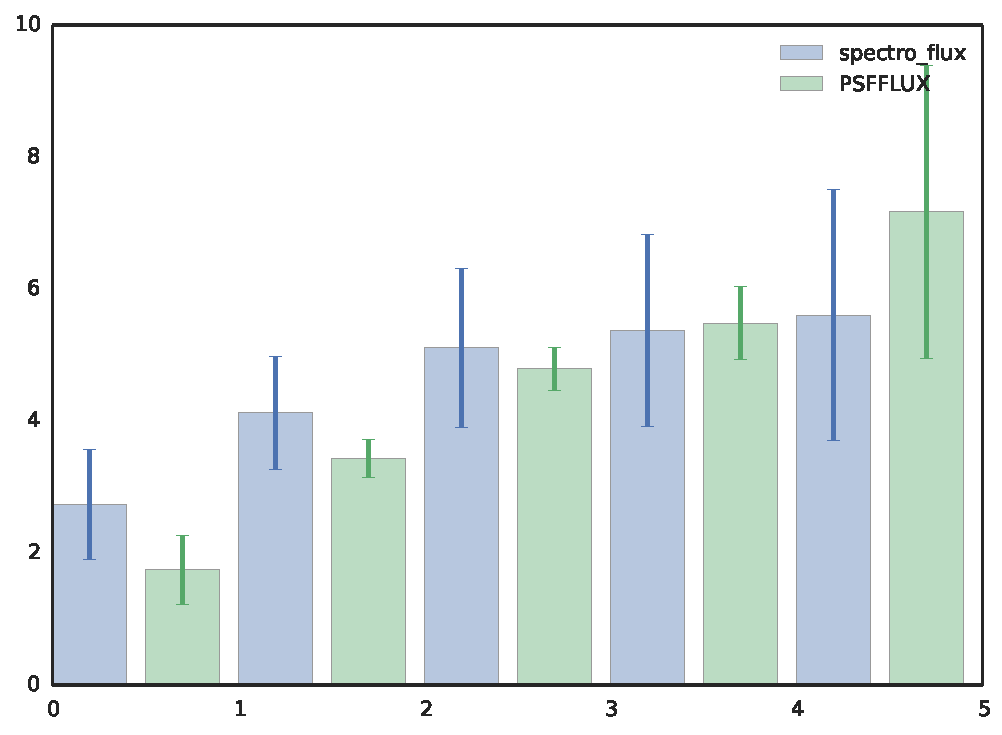
\includegraphics[width=.8\textwidth]{figs/psfflux_vs_spectroflux}

Above is a comparison of the SPECTROSYNFLUX (+ IVAR) and the PSFFLUX (+ IVAR) with two standard errors.  There is a discrepancy - which should I take as true?  How are PSFFLUX measured?  

\end{itemize}


%Questions for David: 
%\begin{itemize}
%\item How to deal with luminosity/distance and the SDSS fluxes.  Can I just assume a spectral %density with arbitrary units $f(\cdot)$ that integrates to one, and this defines the distribution over colors (like normalized SDSS fluxes)?  What's a simple physical model to go from object spectra to SDSS fluxes?
%\end{itemize}


%-- section ------------------------------------------------------------------
%\section{Introduction}
%%%We study the problem of photon 
%
%To discuss
%\begin{itemize} \itemsep 0pt 
%\item The unknown spectrum of a star, quasar or galaxy carries a lot of information 
%\item This spectrum, however, is largely inaccessible for most objects
%\item Astronomical photometry, on the other hand, is much easier to deploy and obtain for a much larger number of sources
%\item Given photometric images of a Quasar, what can we infer about the full spectrum of the object? 
%\item How can we leverage a database of full spectral measurements of many quasars to more accurately and reliably infer the full spectrum?
%\end{itemize}

\section{Related work}
Below is a list of astronomy references on photo-$z$ with a brief summary of methodology/contribution.  

\begin{itemize}

\item \cite{benitez2000bayesian} presents a thorough summary of Bayesian methods for photometric red-shift estimation from spectral templates (as opposed to the so called empirical method of learning a function from colors to z value, e.g.~with a neural network).  They set up the framework where we are given data $D =\{C, m_0\}$, the colors $C$ (ratio of each band's magnitude to some reference band's magnitude) and the magnitude information of the reference band $m_0$.  The goal is then to infer the distribution $p(z | D)$ using some prior information in the form of a spectral template library.  Some interesting notes
  \begin{itemize}
  \item The prior probability $p(z | m_0)$ should be a function of the magnitude of observations (fainter = farther a priori).  They also note that this should be defined in terms of $p(z | \hat m_0)$, where $\hat m_0$ is the true value of that magnitude, and we observe some noisy version that needs to be integrated over.  
  \item They then discuss galaxy templates, $T$, which are essentially types of galaxies (characterized by spectral density).  The fully Bayesian photo-z distribution averages over these templates
  \begin{align}
  p(z | C, m_0) 
    &= \sum_T p(z, T | C, m_0) \\
    &\propto \sum_T p(z, T |m_0) p(C | z, T) \\
    p(z, T | m_0) &= p(T | m_0) p(z | T, m_0)
  \end{align}
  The idea is to then extend $T$ to parameterize the types of spectra expected - basically the weights involved
  \begin{align}
    p(z | C, m_0) &= \int dS p(z, S | C, m_0) \\
     &\propto \int dS p(z, S | m_0) p(C | z, S)
  \end{align}
  where $S$ are like pca weights or other parameters of spectra.  
  \todo{How is $p(C | z, S)$ defined - this is the important part of the likelihood}
  They discuss how to do this with the template idea, but not so much on the parameterization of spectra.  This is the key piece of information I'm missing, and would be the novel contribution of the paper.  
  \item They employ the template method as their likelihood.  The likelihood, if I understand it correctly, looks like this 
  \begin{align}
  p(C | z, T) &\propto 
    \frac{1}{\sqrt{F_{TT}(z)}} 
    \exp \left( -\frac{1}{2} \sum_{\alpha} \frac{ (f_\alpha - a f_{T_\alpha})^2 }{\sigma^2_{f_\alpha}} \right)
  \end{align}
  where $f_{0}, \dots, f_{n_C}$ are the observed fluxes, $f_T{\alpha}(z)$ is the flux of the template $T$ (I think), and $a$ is a magnitude nuisance parameter.  They then discuss different algebraic representations of this likelihood.  
  Importantly, I think their relationship between spectral template $T$ and likelihood $p(\text{fluxes} | z, T)$ is sort of empirical, based on how well individual template fluxes match the observed fluxes.  I think what I need is the function to go from spectral template and red shift to fluxes.  
  \begin{align}
    (f_{T,u},  f_{T, g}, \dots, f_{T, z}) &= h(z, T)
  \end{align}
  or better yet, a parameterization 
  \begin{align}
    f(s, z)_{u}, \dots, f(s, z)_{z} &= h(z, s)
  \end{align}
  where $s$ are like PCA coefficients or other model parameters of the spectra.  

  \item Equation 22 gives the form of the prior they use for the probability of galaxy type given magnitude of reference flux
  \begin{align}
  p(T | m_0) = f_t \exp \left( -k_t(m_0 - 20) \right)
  \end{align}
  
  \item Equation 23 gives the prior probability distribution over red shift given galaxy type and reference flux magnitude 
  \begin{align}
  p(z | T, m_0)
  \end{align}
 
  \end{itemize}

\item \cite{budavari2001photometric} and companion paper \cite{richards2001photometric} goes into specific detail for SED model based photometric redshifts for quasars.  They compare a bunch of methods. In particular, \cite{budavari2001photometric} describes an algorithm for reconstruction a quasar spectrum template from photometric observations and spectroscopic redshifts.  It seems sorta like a dynamic K-means/EM algorithm (they add spectral types as needed), and does a decent job reconstructing bumps where the emission lines are.  

The algorithm is: start with a collection of initial spectral templates (I believe these are rest frame.)  $\psi_1(\lambda), \dots \psi_K(\lambda)$
  \begin{enumerate}
  \item Categorize all photometric observations in the training set into one of these $K$ categories.  Which is the most likely template to describe each observation?
  \item Repair the estimated SEDs of each object (does this mean just de-redshift them?)
  \item Replace each reference templates $\psi_k(\lambda)$ with the mean of each of the repaired templates of that class (discovered in step 1).  This is like computing the new mean in k-means.  
  \item Check to see if you need to add a new template or remove an existing template based on some statistical criterion.  
  \end{enumerate}
  
A difference to point out - my work proposes to do all of these steps within a rigorous probabilistic framework.  We can even incorporate a nonparametric model to add/remove templates (or bases).  Also, my model is more of a factor analysis approach as opposed to clustering.  I'm not sure what difference this makes. 

Some takeaways from this paper: 
  \begin{itemize}
  \item High level intuition: 
    \begin{quote}
    For a given redshift, the photometric observation gives
constraints on the possible underlying SED, since we expect
to get back the measured photometric values by redshifting
the SED and convolving it with the filter response function.
This constraint obviously depends on the photometric
system and, also, the redshift of the object as the rest-frame
spectrum is sampled at different wavelengths.
    \end{quote}
  \item They land on four classes of quasars (Fig 7), each of which has a slightly different distribution of red shift (figure 6)
  \end{itemize}
  Again, this paper doesn't really clarify to me an important aspect - how exactly is the $\chi^2$ objective defined?  How do you go from templates, $T$ to fluxes?  One improvement that I can make would be learning a prior over spectral model weights $w$ (similarly, template indicators $T$), and use this prior to hone in on combinations of $w$ that are likely, while leaving the correlation between $w$ and $z$ alone a priori.  
  Similarly, incorporating prior information about magnitudes might disambiguate really low red shifts with higher red shifts.  

\item \cite{bovy2012photometric} - extreme deconvolution method

\item \cite{suzuki2006quasar} (QUASAR SPECTRUM CLASSIFICATION WITH PRINCIPAL COMPONENT ANALYSIS (PCA): EMISSION LINES IN THE Ly$\alpha$ FOREST)

\item \cite{brescia2013photometric} use a multi-layer perceptron (four layers) regression setting on a combination of SDSS (from the DR7QSO dataset, I believe), UKIDSS, and WISE photometric datasets, comparing photo-z performance on the following intersections:   
  \begin{enumerate}
  \item SDSS: 1.1 $\times$ 105;
  \item SDSS $\cap$ GALEX: 4.5 $\times$ 104;
  \item SDSS $\cap$ UKIDSS: 3.1 $\times$ 104;
  \item SDSS $\cap$ GALEX $\cap$ UKIDSS: 1.5 $\times$ 104;
  \item SDSS $\cap$ GALEX $\cap$ UKIDSS $cap$ WISE: 1.4 $\times$ 104.
  \end{enumerate}
The largest dataset combined 43 features (mostly band fluxes and magnitudes).  
The authors mostly discuss the multi-layer model and their training technique, which is L-BFGS and various rounds of cross validation.   The authors note their model's inability to generalize to regions of the space for which they don't have data (particularly large magnitudes or out of range $z$ values). 

The authors outline a bunch of statistics to compare between methods, including the bias, sample stdev, median of absolute value of two quantities
  \begin{itemize}
  \item $\Delta z = (z_{spec} - z_{phot})$ (residuals) 
  \item $\Delta z_{norm} = (z_{spec} - z_{phot}) / (1 + z_{spec})$ (normalized residuals)
  \end{itemize}
And a bunch of percentages of outliers and such based on those statistics.  One is ``catastrophic outliers'', defined as individual samples where $|z_{norm}| > 2 \sigma(z_{norm})|$ - outside of two sample standard deviations.  

\item \cite{kind2014somz} perform photo-z on a galaxy sample in a two step process\begin{itemize}
\item use a self-organizing map as an unsupervised preprocessing step to put data on a low (2) dimensional manifold, typically from galaxy meta information like fluxes and profile information.  In a sense, galaxies are clustered into little grid cells on this low-dimensional manifold, which are continuous.  
\item Spectroscopic $z$ measurements are then somehow assigned to each grid cell for use in the prediction task.  Prediction seems to be take galaxy features, map it to the cell, and use some sort of average or statistic of that cell's photo-z measurement.  This seems like a $k-nn$ kinda thing?  I'm not sure.  
\end{itemize}
They really emphasize the fact that their SOM is unsupervised, and I'm not sure why it's a selling point.  They deliberately cut off their representation learning step from the actual signal they wish to predict, though it does show the representation is capturing relevant structure.  

Though similar in spirit, the self-organizing map doesn't elicit much of a generative or physical interpretation, and really serves as more of a manifold learning.  I would not expect generalization outside of the range of $z$ values and flux magnitudes to predict accurately with this method.  

\item \cite{budavari2009unified} (Unified photo-z paper)

\item \cite{berk2001composite} Describes a composite spectra for quasars using 2200 sample spectra form the SDSS sample in 2001.  This paper goes into details about the characteristic emission lines and how they combined (de-redshifted, re-binned, took the median, etc), and what it says about the physical makeup of the object. Major quote
  \begin{quote}
  The steps required to generate a composite quasar spectrum involve selecting the input spectra, determining accurate redshifts, rebinning the spectra to the rest frame, scaling or normalizing the spectra, and stacking the spectra into the final composite. Each of these steps can have many variations, and their effect on the resulting spectrum can be significant
  \end{quote}
Takeaway: details about the particular meaning behind emission lines or inductive biases about smoothness or good models for quasar spectra can probably be mined from this paper.  

\item \cite{walcher2011fitting} provides an extensive review of spectral energy density (SED) models for stars and galaxies, and various models and methods that can be used for measuring specific properties.  They describe various types of eigendecomposition of galaxy spectra (SVD, trimmed SVD, robust SVD), and various other models of spectra.  They also go into detail about the emission/absorption lines.  

One example they go into detail is photometric red shifts.  

\begin{quote}
Traditionally, photometric redshift estimation is broadly split into two areas: empirical methods and the template- fitting approach. Empirical methods use a subsample of the photometric survey with spectroscopically-measured red- shifts as a ‘training set’ for the redshift estimators. This sub- sample describes the redshift distribution in magnitude and colour space empirically and is used then to calibrate this relation. Template methods use libraries of either observed spectra of galaxies exterior to the survey or model SEDs (as described in Sect. 2). As these are full spectra, the templates can be shifted to any redshift and then convolved with the transmission curves of the filters used in the photometric survey to create the template set for the redshift estimators.
\end{quote}

\item \cite{ball2008robust} Is cited in the review \cite{walcher2011fitting} as a quasar photo-z method using artificial neural networks.  

\item \cite{myers2009incorporating}

\item \cite{ball2008galaxy}
\end{itemize}

\subsection{Related work takeaways}

This work extends previous work by 
\begin{itemize}
\item Being fully Bayesian - the stochastic process prior allows for integrating out the templates as well - instead of computing $p(z | f, T)$ we marginalize this and compute
\begin{align}
  p(z | f) = \int_T p(T) p(z | f, T) 
\end{align}

\item \todo{Ambitious...} We also make our model directly a function of PIXELS - instead of fitting a flux vector, $f_{ugriz}$ we integrate it out (which includes integrating out location, magnitude, etc).    
\begin{align}
  p(z | x_n, \mathbf{X}) &= \int_{T, f} p(T) p(f | x_n, T) p(z | f, T) \\
  p(z | x_n, \mathbf{X}) &= \int_{\mathcal{W}, \mathcal{B}} p(w | x_n, B) p(B | X, x_n) p(z | w, B, x_n)
\end{align}

In doing this - do we get more realistic uncertainty?  We seem to be underestimating uncertainty quite a bit.  

\item Our model is not a clustering/single type model.  It is a (nonnegative) latent factor model, so we parameterize more of a continuum of types.  Our positive basis also elicits an interpretable basis.  



\end{itemize}





%-----------------------------------------------------------------------------
%-- Outline the model                             ----------------------------
%-----------------------------------------------------------------------------
\section{Stochastic process model of spectra}

Our approach is to directly model the probability distribution over the full spectrum of a quasar given a small number of photometric observations (bands).  We view the spectrum of a quasar as a (scaled) probability distribution itself, and thus model it as a random measure.  Specifically, we specify a model for the \emph{rest frame} spectrum of a quasar, and explain observations by warping the input measurements by the appropriate red-shift values. 

We further assume that each quasar is at some specific red-shift with respect to Earth, $z_n$, (typically in the range 0 to 8).  Denoting the rest-frame spectrum of a quasar $n$ as a function, $f_n^{(rest)} : \mathcal{W} \rightarrow \R_+$, the affect of red-shift on our observations is summarized by the relationship 

\begin{align}
  f_n^{(obs)}(\lambda) &= f_n^{(rest)}(\lambda \cdot (1 + z_n))
\end{align}

\red{There has to be a scaling factor here (otherwise I think energy is not conserved), but I believe I can brush the details under the rug by referring to these as spectral energy densities and say they integrate to 1.}

As the spectrum of a source characterizes much of the information of interest, we take special care creating a structured prior over $f_n(\cdot)$ using available observations of rich spectra. Furthermore, due to the fact that the red-shift value effectively scales the input of this function, we cannot rely on a fixed grid of $\lambda_1, \dots, \lambda_P$ values, but must define a stochastic process to coherently define a probabilistic model.  The rest of this section outlines a model for these spectra and subsequent photometric observations.  

%-- example quasar spectra and redshift -------------------------------
\begin{figure}[t!]
\begin{center}
\begin{subfigure}[a]{.99\textwidth}
  \includegraphics[width=\textwidth]{{"figs/quasar_redshift_obs_frame"}}
  \caption{Observation frame}
\end{subfigure}
\begin{subfigure}[a]{.99\textwidth}
  \includegraphics[width=\textwidth]{{"figs/quasar_redshift_rest_frame"}}
  \caption{Rest frame}
\end{subfigure}
\end{center}
\caption{High fidelity spectroscopy of multiple quasars at different red-shifts, $z$.  The top graphic depicts the spectrograph in the observation frame, which can be intuitively thought of as ``stretched'' by a factor $(1+z)$.  The lower figure depicts the ``de-redshifted'' version of the same quasar spectra.  This effectively squashes observations, and reconstructs the quasar spectra as it would be seen in the quasar's rest frame.  The salient feature of this operation is the alignment of the emission and absorption lines (albeit at different scales).  This alignment will provide the information about $z$ that we can infer from SDSS photometric projections of the very same spectra.}
\label{fig:bands}
\end{figure}


%-----------------------------------------------------------------------------
%-- low rank spectra model                        ----------------------------
%-----------------------------------------------------------------------------
\subsection{Additive stochastic process prior}

% ---- SDSS FILTER FIGURE --------------
\begin{figure}[t!]
\begin{center}
\includegraphics[width=.99\textwidth]{{"figs/quasar_spectrum_sdss_filters"}}
\end{center}
\caption{Example of a (scaled) quasar spectrum with SDSS \emph{ugriz} band filters, $S_{\beta}(\lambda)$, overlaid.  Computing red-shift given the full spectrum is often straightforward and often quite precise, however full spectra are more difficult to obtain.  Photometry data, while far easier to obtain, only measures band specific flux, a weighted average of of the unobserved spectrum of the object. }
\label{fig:filters}
\end{figure}

To model the full spectral observations, we define a library of $K$ latent positive stochastic processes, and assume that the true \emph{rest frame} spectrum is a positive linear combination of these $K$ processes. Spectral observations, $x_n(\lambda_i)$, are measured with Gaussian noise (which can be negative) centered around a realization of the true spectra process.  The noise of the spectral intensity measured at each wavelength is measured and assumed to be known.  The full generative model for this prior is simply 
\begin{align}
  B_k(\cdot) &\sim F_B \text{ with } B_k : \mathcal{W} \rightarrow \R_+ \text{ and } \int_\mathcal{W} B_k(d\lambda) = 1 \\
  f_n(\cdot) &= \sum_{k=1} w_{n,k} B_k(\cdot) \\
  z_n        &\sim F_z \\
  x_n(\lambda_i) &\sim \mathcal{N}\left( f_n(\lambda_i \cdot (1 + z_n)), \sigma^2_{n, \lambda_i}\right)
\end{align}
where $F_B$ defines the probability distribution over the stochastic processes that compose our basis, $B_1, \dots, B_K$, and thus encode assumptions about the overall shape and smoothness of the rest frame spectrum.  The red-shift parameter $z_n$ is drawn from a prior with probability distribution $F_z$.  The observation noise for spectrum $n$ measured at observation wavelength $\lambda_i$ is given by $\sigma^2_{n, \lambda_i}$, and is known.  

We note that this is a similar set up to \red{(cite NMF, LDA, other positive density model stuff here)}, and is an example of a hierarchical mixture model to define a density.  

%-----------------------------------------------------------------------------
%-- spectra => fluxes model                       ----------------------------
%-----------------------------------------------------------------------------
\subsection{Generative model of photometric observations}

%---------------------------------------
\begin{figure}[t!]
\begin{center}
\includegraphics[width=.5\textwidth]{{"figs/quasar_sdss_fluxes"}}
\end{center}
\caption{Flux distributions in the SDSS \textrm{ugriz} bands (columns) computed from high fidelity spectroscopy of four quasars (rows).  The value in each square is computed by integrating the filter band from~\ref{fig:filters} against the full spectrum of the source.  The ``photo-z'' goal is to somehow infer the red-shift of a quasar from these five values spatially distributed in an image. }
\label{fig:fluxes}
\end{figure}

Photometric observations are far less information rich than the full spectrum - fine details are averaged away over large swaths of wavelength values.  However, the band-specific fluxes captured in photometric images do convey information about the object depicted \red{ (cite photo z papers) }.  The photometric count observations can be modeled as a function of the object's unobserved full spectral density in a generative way.  For quasar $n$, the generative process of a photometric observation of a quasar is 
\begin{itemize}
\item Rest-frame quasar spectra is sampled from the structured prior determined by the unsupervised procedure. 
\begin{align}
  f_n(\cdot) &\sim F
\end{align}
or, in the positive basis representation
\begin{align}
  w_{n,k} &\sim p_k(w) \text{ for } k = 1, \dots, K \\
  f_n(\cdot) &= \sum_{k=1}^K w_{n,k} B_k(\cdot)
\end{align}

This defines the amount of energy $W / m^2 / \lambda$ emitted by the quasar.  
\red{Figure out how this relates to the spectral radiance defined by Planck's law.  Figure out how the emission angle portion of Planck's law will relate to this.}.  

\item Red shift is sampled from an appropriate prior \red{(to be determined)}
\begin{align}
  z_n &\sim F_z
\end{align}

\item The number of photons captured in band $\beta$ is a function of the band sensitivity function $S_\beta(\cdot)$, the distance to the object, and the number of photons emitted across the spectrum, given by the photon-energy relationship
\begin{align}
E(\lambda) = \frac{hc}{\lambda} \text{ J / photon }
\end{align}
\red{How does this look to us?  Does it make sense to just stretch out the $f_n(\cdot)$ and then apply $E(\lambda)$, or is there something else that happens that makes this order of operations invalid?}

The expected number of photons measured in band $\beta$ with lens size $A$ m$^2$ and exposure duration $\Delta$ seconds is
\begin{align}
  \mu_{n} &= 
    \underbrace{ b_n }_{ m^2 }
    \underbrace{ \frac{A \Delta}{4 \pi d_n^2} }_{ s }  
    \int_{\Lambda}
    \underbrace{ f_n(\lambda \cdot ( 1 + z_n ))}_{10^{-20} \frac{J}{s \cdot m^2 \cdot \angstrom} }
    \underbrace{ E(\lambda)^{-1} }_{ \frac{photon}{J} }
    S_{\beta_n}(\lambda) d\lambda
\end{align}
where the term $\frac{A \Delta}{4 \pi d_n^2}$ captures the notion that only a small fraction of the shell of radius $d_n$ is being measured.  The $b_s$ term indicates the surface area of emission.  Both $d_n$ and $b_n$ are not measurable, and treated as nuisance variables.  The rest frame spectrum has been shifted to observation frame using the unknown red-shift value $z_n$.  



\item As the spatial appearance of a quasar is modeled as a point source, pixel observations are finally determined by the point spread function, which scatter's light across the lens.   
%In an ideal model, an image of a single point source would only illuminate a single pixel if its light were not scattered on the lens during capture according to the image's point spread function.  
This function, which is assumed known and denoted as $p_n(\cdot)$, models atmospheric effects and other causes of spatial spread of a source's light.  Given the object's expected photon flux, $b_{n, \beta_n}$ (photons / second), the number of photons observed in pixel $n$ in image $n$ is distributed
 
Defining notation, for image $n \in \{1, \dots, N\}$, denote the image band as $\beta_n \in \{u, g, r, i, z\}$, and denote pixel $m \in \{1, \dots, M_n\}$ as $x_{n,m}$. 
\begin{align}
  x_{n,m} &\sim \textrm{Pois}( \mu_n p_n(m) )
\end{align}

\end{itemize}

This defines our likelihood, and our inferential goal is now to compute the posterior distribution over $w_n$ and $z_n$ given the band fluxes.  

\subsection{Inference}

For each image, we sum over all pixels in the spatial extent of the quasar (due to the point spread function).  Due to additive properties of Poissons, this value is distributed
\begin{align}
  \sum_{m}^{M_n} x_{n,m} &\sim \textrm{Pois}\left( b_{n, \beta_n} \sum_{m}^{M_n} p_n(m) \right) \\
    &\sim \textrm{Pois}\left( b_{n, \beta_n} \right) 
\end{align}

Current inference scheme is 
\begin{itemize}
\item Map estimation of $\hat B$ and $\hat W$ a large range of canonical values $\lambda_0$
\begin{align}
  \hat B, \hat W &= 
    \argmax_{B, W} \sum_{n=1}^N \sum_{p = 1}^P p(x_n(\lambda_i) | W_n, B, \sigma^2_n)
\end{align}

\item Full Bayesian inference of $z_n, w_n$ for test $n$.  
We generate posterior samples from the posterior distribution 
\begin{align}
  p(w_n, z_n | B, b_{n, ugriz})
    &\propto \prod_{\beta \in \{ugriz\}} p(b_{n, \beta} | w_n, z_n, B) p(w_n, z_n) \\
    &\propto \prod_{\beta \in \{ugriz\}} p_{pois}\left(b_{n, \beta}; \int_\mathcal{W} S_\beta(\lambda) w_n^\trans B (1 + z_n)) d\lambda \right) p(w_n, z_n)
\end{align}
where the input warping of $w_n^\trans B$ is done by linear interpolation.  This doesn't feel right.  

\red{ This is also currently done by univariate slice sampling.  This is super slow, and I'm not sure how well it's converging. }

\end{itemize}

\subsection{Data}
We use a database of full spectral measurements and precisely measured red-shifts to predict quasars for which we only have photometry data (\red{ where do these specifically come from? }).  

We observe noisy measurements of the full spectra, $y_n$, (quasar $n$ of $N$) recorded on a wavelength grid $\Lambda = (\lambda_1, \dots, \lambda_P)$.  The values of $y_n$ have been perturbed by Gaussian noise $\sigma_n$ (and thus, can be negative), however we know that the spectral distribution of light must be positive, so we assume there is some latent spectrum $f_n$ that specifies $y_n$.  Precisely, this relationship can be written
\begin{align}
  y_n &\equiv (y_{n, \lambda_1}, \dots, y_{n, \lambda_P}) \text{ for } n = 1, \dots, N \\
  \sigma_n^2 &\equiv (\sigma_{n, \lambda_1}^2, \dots, \sigma_{n, \lambda_P}^2) \\
  y_{n, \lambda_1} &\sim \mathcal{N}(f_n(\lambda_1), \textrm{diag}(\sigma_{n}))
\end{align}

We approach this task as a density estimation problem, where we find a physically interpretable low-dimensional specification of a quasar's spectral density.  


%-------------------------------------
\begin{figure}[t!]
\begin{center}
\includegraphics[width=.95\textwidth]{{"figs/quasar_spectrum_ivar"}}
\end{center}
\caption{Example of measured quasar spectrum (blue), $x_{n, \lambda_p}$, and inverse variance of the measurement (grey), $\sigma_{n, \lambda_p}^{-2}$. }
\label{fig:fluxes}
\end{figure}


%-- section --------------------------------------------------------
\section{Experiments} 

We run several experiments to show the utility of this model.  We divide the $N = 568$ available spectra and their precisely measured $z$ values into a training set, $N_{train} = 400$, and a testing set, $N_{test} = 168$.  We then take the testing set, and project the full spectra down on to the SDSS bands by numerically integrating the test spectra against the known filter sensitivities.  These serve as ``test fluxes'' from which we predict red-shift and validate our model.  

Our experimental framework proceeds as follows
\begin{itemize}
\item Fit a model over the training set, $\hat B, \hat W$
\item For each quasar $n$ in the test set
  \begin{itemize}
  \item Compute band fluxes, $b_{n, \beta}$ for the SDSS $ugriz$ bands.  
  \item Compute posterior samples of $z_n, w_n | b_{n, \beta}, B$
  \item Predict with the expectation of the posterior marginal distribution: 
  \begin{align}
    z_n = E\left(z_n | b_{n, \beta}, B\right)
  \end{align}
  \end{itemize}
\end{itemize}

\subsection{Non-negative basis decomposition}

Figure~\ref{fig:basis} graphically depicts the non-negative basis decomposition, $B_1, \dots, B_k$, from 400 quasar spectra, and Figure~\ref{fig:reconstruction} depicts the model's reconstruction for one quasar.  

%-----------------------------------------------------------
\begin{figure}[t!]
\begin{center}
\begin{subfigure}[a]{.99\textwidth}
\includegraphics[width=.99\textwidth]{{"figs/rank_4_basis"}}
  \caption{Basis}
  \label{fig:basis}
\end{subfigure}
\begin{subfigure}[a]{.99\textwidth}
  \includegraphics[width=\textwidth]{{"figs/idx_0_rank_4_reconstruction"}}
  \caption{Example Reconstruction}
  \label{fig:reconstruction}
\end{subfigure}
\end{center}
\caption{The upper plot depicts the non-negative basis decomposition of 400 rest frame quasar spectra (de-redshifted) from a maximum a posteriori fit to the model.  The lower plot shows an example reconstruction of one quasar in red.}
\label{fig:bands}
\end{figure}

\subsection{Photo-z measurements}

Figure~\ref{fig:posterior} depicts a sampling of marginal posterior distributions of $z_n$ conditioned only on band fluxes and the learned basis $B$.  

Figure~\ref{fig:recon} depicts the reconstruction of the full spectra from the five band fluxes $b_{n, \beta}$.  

Figure~\ref{fig:prediction} depicts the ``photo-z'' prediction against the spectroscopic measurement of red-shift for the held out test stars.  


%------------------------------------------------------------------
\begin{figure}[t!]
\begin{center}
\begin{subfigure}[a]{.45\textwidth}
  \includegraphics[width=\textwidth]{{"figs/quasar_plots/quasar_109_posterior_z"}}
\end{subfigure}
\begin{subfigure}[a]{.45\textwidth}
  \includegraphics[width=\textwidth]{{"figs/quasar_plots/quasar_112_posterior_z"}}
\end{subfigure}
\begin{subfigure}[a]{.45\textwidth}
  \includegraphics[width=\textwidth]{{"figs/quasar_plots/quasar_68_posterior_z"}}
\end{subfigure}
\begin{subfigure}[a]{.45\textwidth}
  \includegraphics[width=\textwidth]{{"figs/quasar_plots/quasar_155_posterior_z"}}
\end{subfigure}
\begin{subfigure}[a]{.45\textwidth}
  \includegraphics[width=\textwidth]{{"figs/quasar_plots/quasar_164_posterior_z"}}
\end{subfigure}
\begin{subfigure}[a]{.45\textwidth}
  \includegraphics[width=\textwidth]{{"figs/quasar_plots/quasar_73_posterior_z"}}
\end{subfigure}
\end{center}
\caption{Histogram of red-shift posterior samples given only the SDSS band projection of the full spectrum.  These histograms were computed with 5,000 MCMC samples (after 5,000 burn-in) using slice sampling.  The full spectrum measured red-shift is the vertical black line, and the posterior expectation of the red-shift is the vertical red line. }
\label{fig:posterior}
\end{figure}

\begin{figure}[t!]
\begin{center}
\includegraphics[width=.75\textwidth]{{"figs/red-shift-test-predictions"}}
\end{center}
\caption{Red-shift predictions for 167 held out test Quasars and posterior dispersion.  \red{What the hell is going on with that weird under estimation cluster???} }
\label{fig:prediction}
\end{figure}


%------------------------------------------------------------------
\begin{figure}[t!]
\begin{center}
\begin{subfigure}[a]{.7\textwidth}
  \includegraphics[width=\textwidth]{{"figs/quasar_plots/quasar_109_mcmc_recon"}}
  \caption{u band}
\end{subfigure}
\begin{subfigure}[a]{.28\textwidth}
  \includegraphics[width=\textwidth]{{"figs/quasar_plots/quasar_109_posterior_z"}}
\end{subfigure}

\begin{subfigure}[a]{.7\textwidth}
  \includegraphics[width=\textwidth]{{"figs/quasar_plots/quasar_112_mcmc_recon"}}
  \caption{g band}
\end{subfigure}
\begin{subfigure}[a]{.28\textwidth}
  \includegraphics[width=\textwidth]{{"figs/quasar_plots/quasar_112_posterior_z"}}
\end{subfigure}
\end{center}
\caption{Monte Carlo reconstruction of the full spectrum from the five band test fluxes. The green line is the posterior median (at wavelength) and the grey lines are the 1st and 99th percentile samples.  On the right are the respective red-shift posterior distributions.  \red{There seems to be some bias to the right (over prediction) in the upper cluster} }
\label{fig:recon}
\end{figure}


\begin{figure}[t!]
\begin{center}
\includegraphics[width=.75\textwidth]{{"figs/weight_pca_rank_4"}}
\end{center}
\caption{PCA projection of $\log w_n$ to two dimensions. \red{Examine the $z$ values, appearances, and total flux of the big cluster versus the outliers} }
\label{fig:prediction}
\end{figure}


\clearpage
\bibliographystyle{plainnat}
\bibliography{refs}
\end{document}